\section{Analyzer}

The analyzer is a static analysis system built for PyTorch. As PyTorch is a dynamic-graph-based machine learning framework, it is difficult to obtain the graph information before execution. Our analyzer is built upon the PyTorch FX module~\cite{torch-fx} to obtain the static computation graph ahead of time. 

The analyzer consists of three parts: a \textit{symbolic profiler} for collecting computing and memory overhead related to static computation graph, a \textit{cluster detector} for collecting hardware characteristics and detecting cluster topology, and a \textit{tensor layout manager} to find efficient tensor layout conversion the path from different sharding spec and record conversion cost.\par

\subsection{Symbolic Profiler}

% \textit{Symbolic profiler} obtains the static computation graph of the model through symbolic tracing. We improved upon the PyTorch FX~\cite{torch-fx} symbolic tracing to support a wider range of operations and control flow.
% The analyzer annotates the meta information for each node during graph tracing, and collects both the computing overhead (TFLOPs) and memory overhead (Byte) for all feasible intra-op parallel strategies of each node using symbolic execution. The symbolic execution is achieved with PyTorch meta tensor and the operation only computes the meta data of the output such as shape and data type. Therefore, the overhead of the symbolic profiling process is negligible.\par

In order to evaluate the best strategies for parallelization and activation checkpoint, we need to obtain information such as the number of floating point operations and memory consumption. However, as PyTorch is a machine learning framework based on dynamic graph execution, such information is generally collected during runtime, imposing a significant challenge to our search.

With the latest PyTorch FX ~\cite{torch-fx} module, this becomes possible with symbolic tracing. Symbolic tracing does not conduct real computation, instead, it only infers the output's meta data such as shape and data type as shown in figure~\ref{fig: symbolic}. We improved upon the PyTorch FX~\cite{torch-fx} symbolic tracing to support a wider range of operations, control flow, and PyTorch meta tensors. During tracing, the analyzer annotates the meta information for each node, and collects both the computing overhead (TFLOPs) and memory overhead (Byte) using symbolic execution.
In this way, since computation is only simulated instead of actually executed, we are able to extract the computation graph and relevant meta information ahead of execution and the overhead of profiling is reasonably low.


\begin{figure}[h]
    \centering
    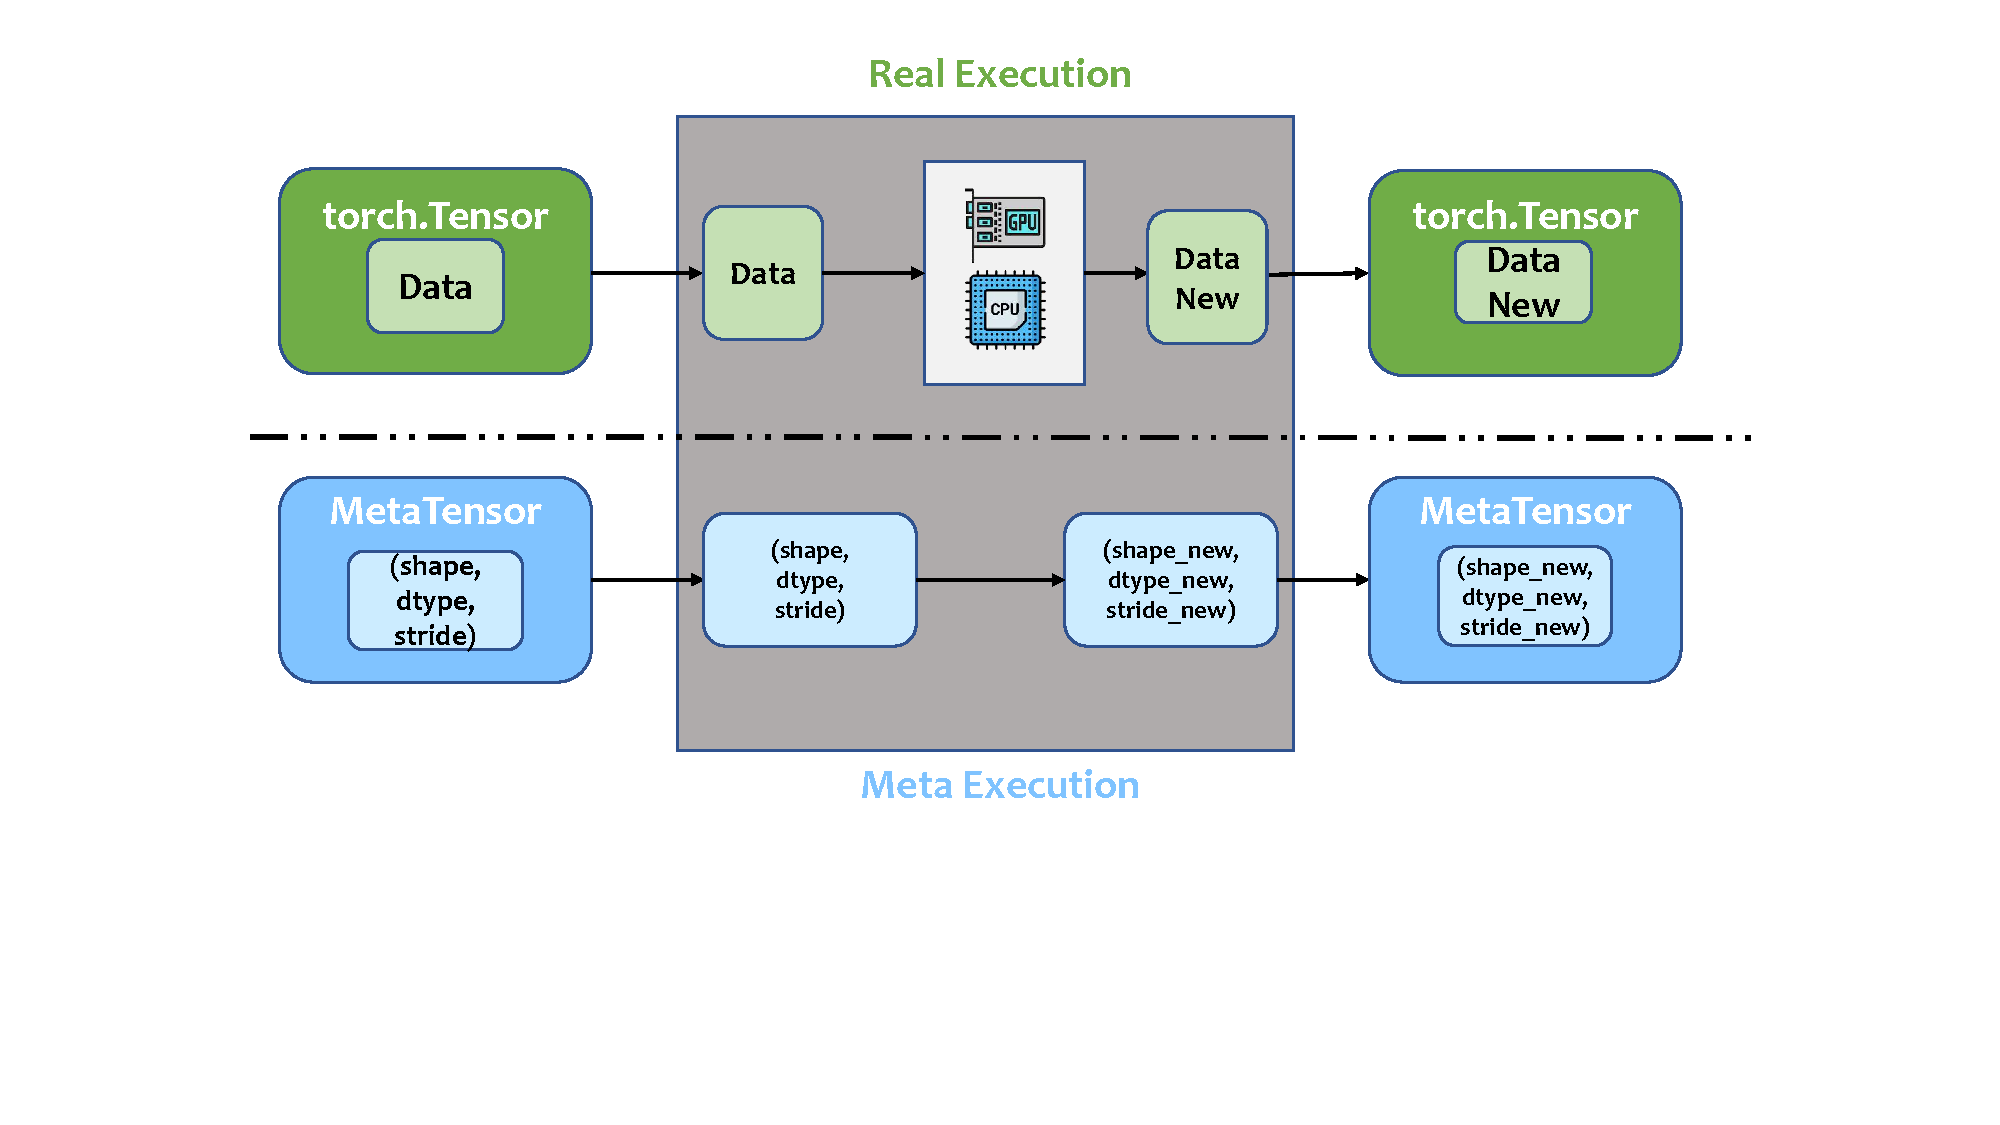
\includegraphics[width=0.5\textwidth]{img/meta_execution.pdf}
    \caption{symbolic execution}
    \label{fig: symbolic}
\end{figure}



% \noindent\textbf{Intermediate representation.}  We used the torch FX graph as our IR (as picture), which is a DAG-based IR. In the FX graph, a node has a string type opcode to describe the op type and an associated target which is the calling target of call nodes (call\_module, call\_function, call\_method). In addition, the node also has arguments and keyword arguments to show data dependencies between nodes.\par

% PyTorch provides a symbolic tracer to obtain this static computation graph symbolically. In our system, in order to better serve our solver, we made some modifications based on the FX tracer. During the tracing, we injected the meta\_data attribute for each node, which records the meta information for the inputs and outputs of nodes, including but not limited to shape, dtype, etc.\par

% \noindent\textbf{Symbolic Profiling.}  In order to provide enough information to search for an optimal parallel strategy, we need to profile the computational overhead and memory overhead of the node. \par In our intra-op parallelism solver, we profile the computational overhead and memory overhead of every legal sharding strategy for each node. If these overheads are profiled one by one using real execution, the tremendous cost of profiling will greatly affect the user experience. Therefore, our profiler needs to ensure that it can use \textit{symbolic execution} as shown in figure~\ref{fig: symbolic}, which means the profiling process run with a tensor that holds no actual memory. \par

% Additionally, the activation checkpoint solver needs further analysis on the autograd graph, which is a finer-grained level of the computation graph. Analysis with lower levels of operators on a complete computation graph (including forward calculation and backpropagation) can be very helpful to figure out the peak memory.\par

% \noindent\textbf{Hacking Autograd.} Under the PyTorch framework, if you want to obtain a complete computational graph with lowered operators of the \textsc{torch.ops.aten}, you can do it by adding operators chosen in the torch dispatching phase to the computation graph. In order to meet the requirements of symbolic execution at the same time, we need to dispatch the operator to the meta backend. However, without breaking the original implementation of the framework, we cannot modify the Autograd selection priorities of different backends in the torch dispatcher selecting phase. Moreover, the device information of the allocated tensors will always be lost, since all of them appear on the meta backend.\par
% In order to solve this problem, we constructed a MetaTensor. From the perspective of the dispatcher, MetaTensor is a fake CPU tensor or a fake CUDA tensor, while at runtime, the PyTorch dispatcher is hacked to unwrap input CPU or CUDA tensor execution into shape inference. After that, the result tensor is generated and re-wrapped as another fake CPU or CUDA tensor. This could cheat the PyTorch dispatcher's inspection so that all of our computations are performed in a symbolic way. Through the method of Hacking Autograd, we meet the requirement of profiling through symbolic execution without losing any generality.\par

% \noindent\textbf{Computing Profiling.} To profile the computing overhead of each node, a corresponding function  is registered to calculate FLOPS for each operator, and the FLOPS counting function of the corresponding operator in the hijacked \_\_torch\_dispatch\_\_. In our implementation, we found that all operators can be divided into five categories: matmul, convolution, reshape, elementwise, and zero. We only need to implement the FLOPS counting functions for these five types, and then register the operators to the corresponding category, which can cover most of the algorithm models.\par



% 先不考虑buffer的版本
% \noindent\textbf{Memory Profiling.} In order to better analyze the fluctuation of memory, we divide the memory overhead of node into two stages, forward and backward, corresponding to \textbf{fwd\_in}, \textbf{fwd\_buffer}, \textbf{fwd\_tmp}, \textbf{fwd\_out}, \textbf{bwd\_out}, \textbf{bwd\_buffer}, \textbf{bwd\_tmp} respectively (as shown in the figure~\ref{fig: memory profiling}). With this information, we can know the memory usage of each node before performing forward calculation or backpropagation. In addition, with fwd\_buffer and bwd\_buffer, we can estimate how much additional memory consumes during node internal computation, as well as the value of the peak memory and which node the peak occurs in.

% % This fig should be renewed
% \begin{figure}[h]
%     \centering
%     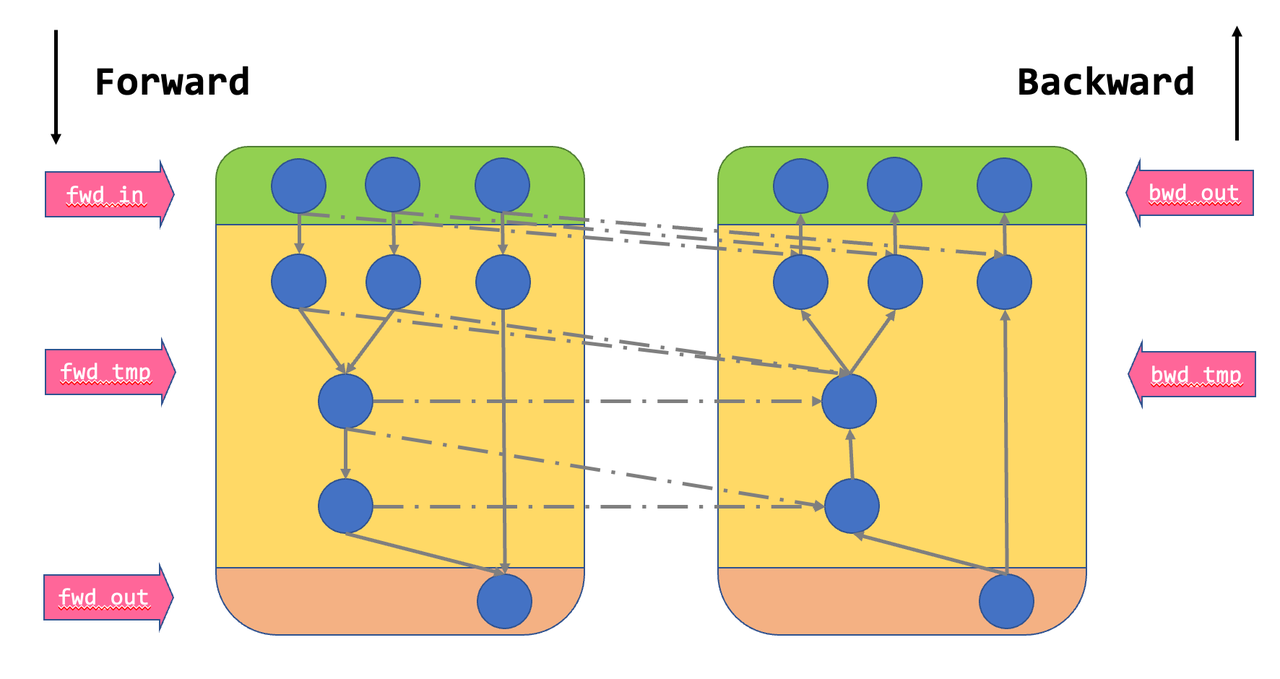
\includegraphics[width=0.5\textwidth]{img/memory_profiling.png}
%     \caption{Memory Profiling}
%     \label{fig: memory profiling}
% \end{figure}

\begin{figure*}[h!]
    \centering
    
\includegraphics[width=0.9\textwidth]{img/overall.png}
    \caption{symbolic memory profiling evaluation}
    \label{fig: evaluation}
\end{figure*}

% \begin{itemize}
% \item \textbf{fwd\_in}: Saves all the tensors which are saved for backward in the forward computation of this operator
% \item \textbf{fwd\_buffer}: Saves all the buffer tensors generated in the forward computation of this operator. If the current operator is checkpointed, these tensors will be released during the forward computation of the operator, but if they are not checkedpointed, then these tensors will be saved until the backward propagation related to this node is complete
% \item \textbf{fwd\_tmp}: The temp tensors generated in the forward computation of this operator. It will be released once the forward operation is done.
% \item \textbf{fwd\_out}: Saves all the output tensors in the forward computation of this operator.
% \item \textbf{bwd\_buffer}: Saves all buffer tensors generated during the backward propagation of this operator.
% \item \textbf{bwd\_tmp}: The temp tensors generated in the backward computation. Similar with \textbf{fwd\_tmp}, it will be released once the backward operation is done.
% \item \textbf{bwd\_out}: Saves the output tensor computed by this operator backward, generally the size of \textbf{bwd\_out} are same as \textbf{fwd\_in}.
% \end{itemize}

% \noindent\textbf{Memory Profiling.} In order to better analyze the fluctuation of memory, we divide the memory overhead of the node into two stages, forward and backward, corresponding to \textbf{fwd\_in}, \textbf{fwd\_tmp}, \textbf{fwd\_out}, \textbf{bwd\_out}, \textbf{bwd\_tmp} respectively (as shown in the figure~\ref{fig: memory profiling}). With this information, we can know the memory usage of each node before performing forward calculation or backpropagation. In addition, with fwd\_buffer and bwd\_buffer, we can estimate how much additional memory consumes during node internal computation, as well as the value of the peak memory and which node the peak occurs in.

% This fig should be renewed
% \begin{figure}[h!]
%     \centering
%     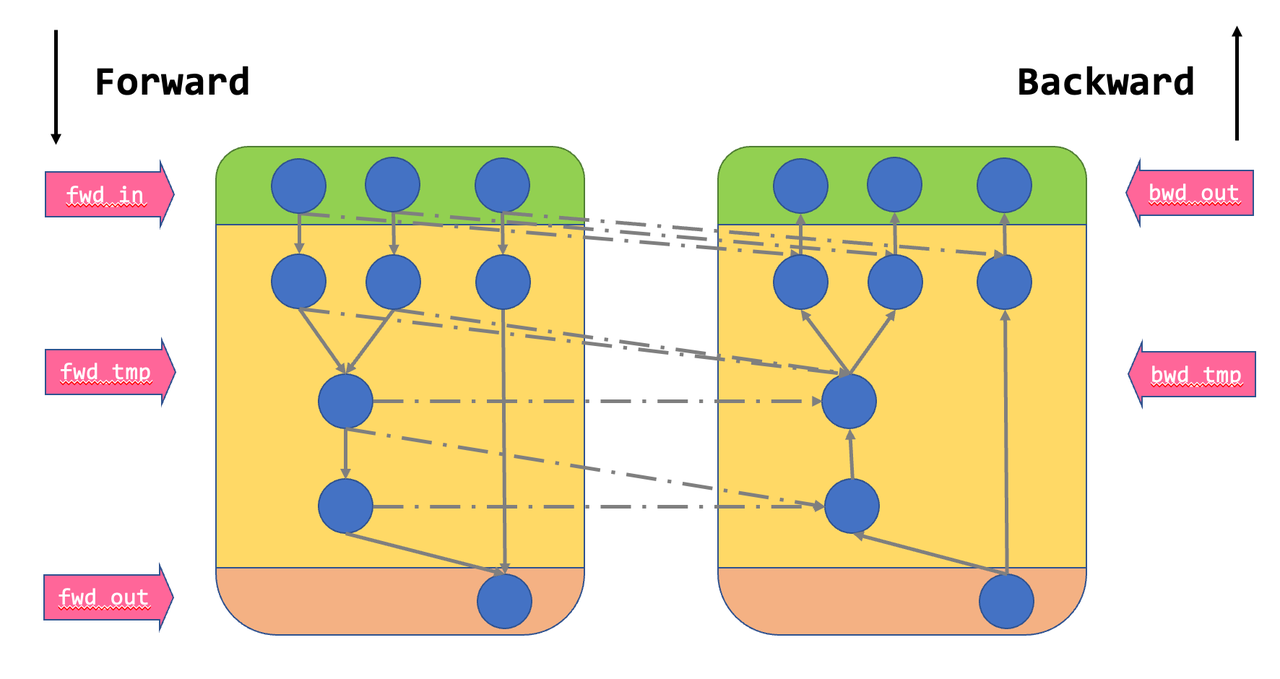
\includegraphics[width=0.5\textwidth]{img/memory_profiling.png}
%     \caption{Memory Profiling}
%     \label{fig: memory profiling}
% \end{figure}



% \begin{itemize}
% \item \textbf{fwd\_in}: Saves all the tensors which are saved for backward in the forward computation of this operator
% \item \textbf{fwd\_tmp}: The temp tensors generated in the forward computation of this operator. It will be released once the forward operation is done.
% \item \textbf{fwd\_out}: Saves all the output tensors in the forward computation of this operator.
% \item \textbf{bwd\_tmp}: The temp tensors generated in the backward computation. Similar to \textbf{fwd\_tmp}, it will be released once the backward operation is done.
% \item \textbf{bwd\_out}: Saves the output tensor computed by this operator backward, generally the size of \textbf{bwd\_out} are same as \textbf{fwd\_in}.
% \end{itemize}
% \begin{figure*}[ht]
%     \centering
%     
\includegraphics[width=0.9\textwidth]{img/overall.png}
%     \caption{symbolic memory profiling evaluation}
%     \label{fig: evaluation}
% \end{figure*}


% \begin{figure}[h!]
%     \centering
%     \begin{subfigure}[t]{0.5\textwidth}
%         \centering
%         
\includegraphics[width=\textwidth]{img/4.png}
%         \caption{}
%         \label{fig: inplace}
%     \end{subfigure}
%     \hfill
%     \begin{subfigure}[t]{0.5\textwidth}
%         \centering
%         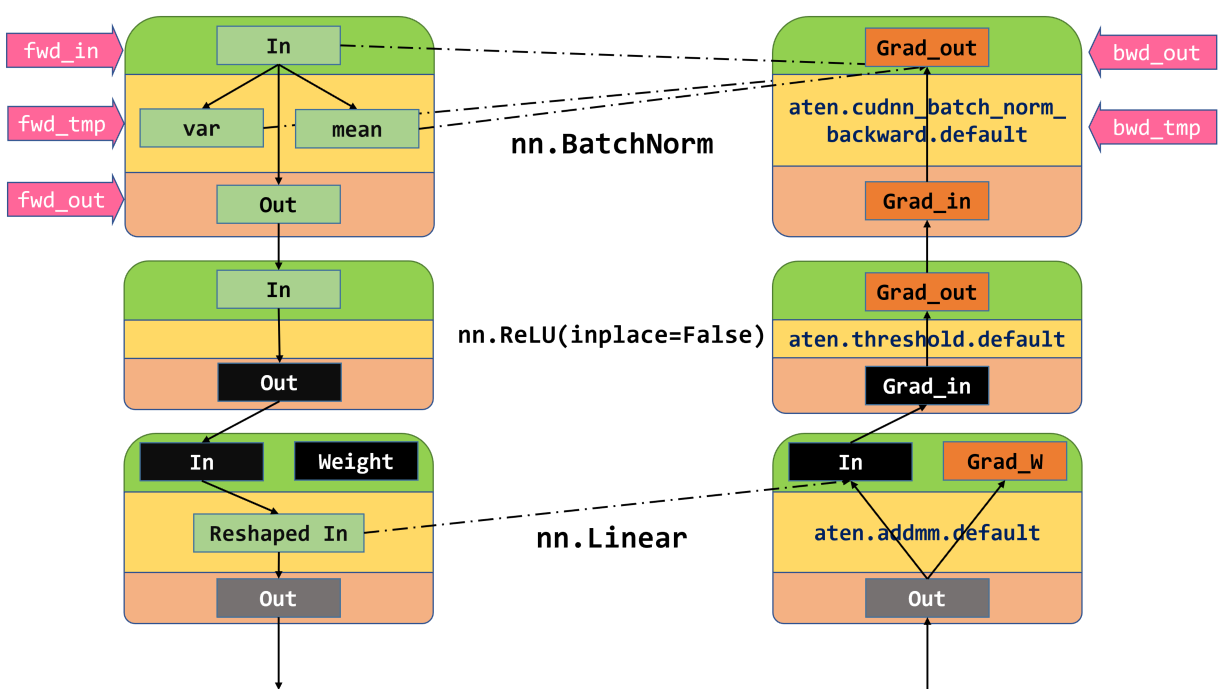
\includegraphics[width=\textwidth]{img/5.png}
%         \caption{}
%         \label{fig: non-inplace}
%     \end{subfigure}
% \end{figure}


% It should be noted that these tensors in fwd\_out will be used as the input of user nodes. To determine which tensors in fwd\_out of the current node are saved, we need to know the configuration of user nodes, such as in-place or not. As shown in the figure, if the in-place setting of the ReLU operator behind BatchNorm is False, the fwd\_out of BatchNorm will be saved. On the contrary, if the in-place setting is True, the fwd\_out of BatchNorm will not be saved.

% \begin{figure}[h]
%     \centering
%     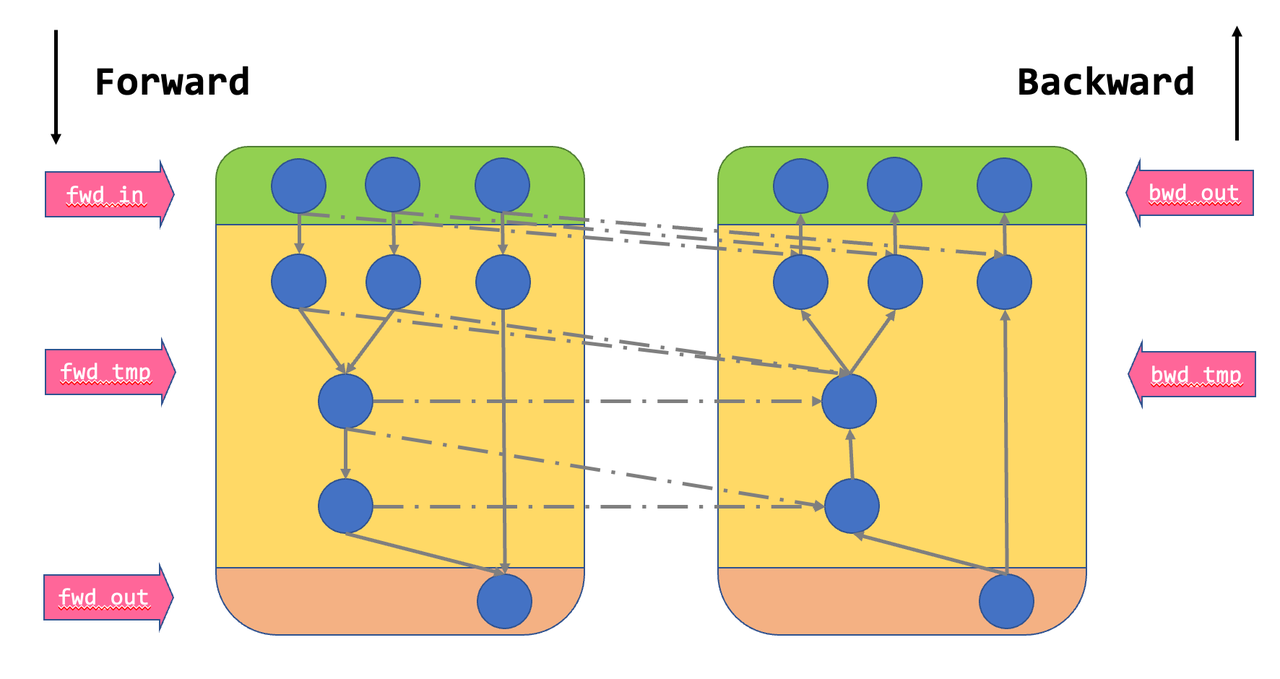
\includegraphics[width=0.5\textwidth]{img/memory_profiling.png}
%     \caption{Memory Profiling}
%     \label{fig: memory profiling}
% \end{figure}

% \noindent\textbf{Evalution.} 

In order to evaluate the accuracy of this profiler, we tested it on more than a dozen mainstream algorithm models including VGG\_16, Resnet50, ViT, GPT2, etc. The memory estimation result is very close to the value of real execution as shown in figure~\ref{fig: evaluation}.


\subsection{Cluster Detector}

We have adopated the concept of device mesh from Alpa~\cite{zheng2022alpa} in our work to have an abstraction for the devices involved in distributed training. The device mesh represents a group of devices as a 2D mesh. For example, 8 physical GPUs can be viewed as 1x8 or 2x4 logical meshes. In the logical device mesh, all computation and collective communication operations will equally occur in each dimension of the device mesh. Therefore, the device mesh need to ensure that devices on the same axis have the same communication performance as each other, otherwise, the device with the lowest bandwidth will slow down the communication process.

Alpa assumes the communication bandwidth between devices in the same computing node are same. However, there are some clusters only have NVLink between 4 pairs of adjacent GPUs. In order to have a better performance, we need to be aware of the fine-grained topology of cluster computing nodes.

To achieve this goal, our cluster detector collects cluster communication performance, such as latency and bandwidth, and detects fine-grained cluster topology. The communication latency is estimated by communicating a series of small-size communication objects in the process group, and the algorithm bandwidth is estimated by communicating large-size communication objects in the process group. With the algorithm bandwidth, the bus bandwidth could be derived through the algorithm bandwidth. With the cluster communication performance, we can deduce the network topology and use it to construct an optimal device mesh where the devices in the same axis have equal communication capability. At the same time, communication performance attributes could be added to the constructed device mesh through the detected cluster information.

\subsection{Tensor Layout Manager}

In intra-op parallelism, a tensor can be sharded into different layouts. Therefore, a representation is needed to describe how a tensor is sharded. We follow Alpa's definition of SMPD-style sharding specifications in our system.
For an N-dimensional Tensor, its sharding spec is to be defined as $X_0X_1...X_{n-1}$, where $X_i$ belongs to {$S$, $R$}, and the representation of this $S$ has a subscript.
If the spec corresponding to $X_i$ is $S_j$, it means that the tensor will be sharded along the $j$th axis of the device mesh in its $i$th dimension. 
In particular, if $S$ has two or more subscripts, it means that the shard will be performed along all subscript axes.

When a tensor is required to have different sharding specs in upstream and downstream operators, we need to perform layout conversion processing, which is called redistribution. There are currently two mainstream methods, enumeration conversion, and dimension-by-dimension conversion. 

Enumeration conversion is to enumerate all possible situations, and then find the corresponding conversion scheme in the table when conversion is required.
However, as the dimension of the device mesh increases, it is difficult to compute the conversion path, and the size of the enumeration is significantly large. 

Dimension-by-dimension conversion is for a convert the sharding spec from its first dimension to the last dimension in the sequence given an N-dimensional tensor. For example, assuming we have a tensor whose sharding spec is $X_0X_1...X_{n-1}$, we need to transform this sharding spec $X'_0X'_1...X'_{n-1}$. We start from the 0th dimension and convert from $X_0$ to $X'_0$ and repeat until the last dimension. In this way, no matter how many dimensions the device mesh and tensor have, a feasible conversion sequence can always be generated. However, the conversion efficiency is poor as it does not guarantee the conversion sequence is optimal.

To tackle these problems, we propose a novel algorithm~\ref{alg: layout conversion}, using heuristic search, to solve the conversion problem of sharding spec, which can be described as:
\begin{enumerate}
    \item Generate all one-step transform sharding specs from source spec
    \item In the one-step transform sharding specs, according to the similarity function, select a sharding spec with the "least difference" as the subsequent source sharding specification, and record the sharding spec in the transform path. If a sharding spec of the one-step transforms is the same as the target sharding spec, the algorithm ends.
    \item Repeat 1, 2 until the end of the algorithm
\end{enumerate}

% \begin{algorithm}
% \caption{layout conversion path}
% % \begin{algorithmic}[1]
% % \State Input: $source\_spec, target\_spec$
% % \State Output: $transform\_path$
% \KwData{$source\_spec, target\_spec$}
% \KwResult{$transform\_path$}

% $total\_step \leftarrow 0$;
% \State $transform\_path(total\_step) \leftarrow source\_spec$
% \Repeat
% \State $min\_diff \leftarrow \infty$
% \State $valid\_transforms \leftarrow \func{Transform}(source\_spec) $
% \ForAll{$sharding\_spec \in valid\_transforms$}
% \State $diff\leftarrow\funcs{Heuristic}(sharding\_spec, target\_spec)$
% \If{$diff < min\_diff$}
% \State $source\_spec \leftarrow sharding\_spec$
% \State $min\_diff \leftarrow diff$
% \EndIf
% \EndFor
% \State $total\_step += 1$
% \State $transform\_path(total\_step) \leftarrow source\_spec$
% \Until{$min\_diff == 0$}
% \State $\Return transform\_path$
\RestyleAlgo{ruled}

\begin{algorithm}[h]
\caption{An algorithm with caption}
\label{alg: layout conversion}
\KwData{$source\_spec, target\_spec$}
\KwResult{$transform\_path$}
$total\_step \leftarrow 0$\;
$transform\_path \leftarrow []$\;
$transform\_path[total\_step] \leftarrow source\_spec$\;
\While{$min\_diff \neq 0$}{
$min\_diff \leftarrow \infty$\;
$valid\_transforms \leftarrow Transform(source\_spec) $\;
\ForAll{$sharding\_spec \in valid\_transforms$}{
$diff\leftarrow Heuristic(sharding\_spec, target\_spec)$\;
\If{$diff < min\_diff$}{
$source\_spec \leftarrow sharding\_spec$\;
$transform\_path(total\_step) \leftarrow source\_spec$\;
}
}
$total\_step \mathrel{+}=  1$\;
$transform\_path(total\_step) \leftarrow source\_spec$\;
}
\Return  $transform\_path$\;
\end{algorithm}

\noindent\textbf{One-step transform.} In our layout manager, there are three operations that will change the sharding spec: all gather, shard, and all to all. All feasible sharding specs derived from each operation's single conversions will be added to the one-step transform sharding spec list. For example, the one-step transform list of $S_0R$ is [$RR$, $S_0S_1$, $S_{01R}$, $RS_0$]. Note that there may be some operations that are not valid here because the sizes of different dimensions of the tensor will be different. If the dim spec of Xi is converted to Sj, and the size of the i-th dimension cannot be divided by the j-th axis of the device mesh size, then this sharding spec is invalid.

\noindent\textbf{Heuristic function.} The rule of the heuristic function we used to measure the difference between two sharding specs dimension by dimension, so the difference between source\_spec and target\_spec can be expressed as\\ 
\begin{center}
$\sum_{\substack{i \in (0, 1, \dotsc,dim(s)-1)}} dim\_diff(s[i], t[i])$.
\end{center}


\textit{Dim difference} will calculate the cost of conversion between dimensions accumulate the cost of all operations, and the final value is the total cost. Note that the overhead here does not refer to the actual time overhead or communication volume of the operation, but is a value used to describe the difference between the two dim specs. The operations that can change the dim spec are all-gather and shard. Because shard is an on-chip operation, and all gather communication takes place cross devices, we need to assign a larger cost to the all-gather operation. In addition, if more than one conversion is required between two dim specs, a step penalty will be imposed. For example, $S_0$ -> $S_1$, the conversion path is $S_0$ -> R -> $S_1$, that is, it needs to perform all gather on the 0th axis of the device mesh, and then perform sharding on the 1st axis of the device mesh, so $dim\_diff(S_0, S_1) = cost(all\_gather) + cost(shard) + step\_penalty.$


\noindent\textbf{Solver supports.} In addition to providing the core functions of the above search, our layout manager records the communication overhead required to convert a tensor from source spec to target spec for layout conversion. This overhead is estimated by the alpha-beta cost model, where the alpha and beta values are obtained from the cluster detector and will be used in both the intra-op parallelism solver and activation checkpoint solver.\par

At the same time, in order to avoid repeated searching at runtime, we use the solved source-target spec pair as the key and the corresponding transform path as the value and put it in a \textit{cache dictionary}. Because our execution plan is fixed at runtime, and the intra-op parallelism solver will calculate the tensor layout converting cost for all possible upstream and downstream sharding spec conversions, we will not do any tensor layout converting search during runtime.